\section{Consideraciones}

% El presente trabajo utiliza la norma APA 6ª edición para la citación de referencias bibliográficas. Todas las citaciones a lo largo del texto utilizan hipervínculos hacia sus entradas correspondientes en \hyperref[chap:referencias]{Referencias bibliográficas} de la página~\pageref{chap:referencias}. 

Muchos términos científicos utilizados se ha optado por escribirlos en inglés\todo{Finalmente he optado por dejar esto aquí en lugar de en nota al pie}, ya que son ampliamente conocidos y usados en su forma original inglesa incluso en el ámbito científico hispanohablante (como \emph{machine learning} o \emph{deep learning}), mientras otros se encuentran en español por haberse considerado la forma más común (como \emph{inteligencia artificial} o \emph{red neuronal artificial}). En todo caso, se ha ofrecido una traducción de todos los términos ingleses en su primer uso para facilitar la lectura. Los términos utilizados repetidamente a lo largo del texto se encuentran en forma de acrónimos, los cuales se han explicitado en su primer uso y en los lugares donde ha sido necesario para mantener la claridad del texto. El desglose de estos acrónimos puede consultarse en el glosario de la página~\pageref{chap:glosario}, a donde apuntan todos ellos por medio de hipervínculos.

Los códigos QR enlazan a recursos complementarios al texto, los cuales pueden cambiar o desaparecer con el tiempo. Por ello, en el anexo \ref{anexo:repositorio} se incluye un enlace al repositorio de GitHub donde se aloja el código fuente en \defaultLaTeX{} de este trabajo, así como los materiales sonoros y de software generados en el marco de este trabajo.

El título de este trabajo hace un guiño a las ya cientos de publicaciones científicas que utilizan la expresión <<All You Need>> en el título (véase la Figura \ref{fig:all_you_need_publicaciones}). Esta expresión se ha convertido en un icono de los avances en \gls{ia}, especialmente desde la publicación en 2017 del emblemático artículo \emph{Attention Is All You Need} \citep{vaswaniAttentionAllYou2017}. El lector curioso puede encontrar una lista actualizada de estas publicaciones en el repositorio de GitHub \emph{Awesome "all you need" papers} \citep{nishiKentoNishiAwesomeallyouneedpapers2024}. En el mismo sentido, los epígrafes de los capítulos son algunos de estos títulos, escogidos sin más pretensión que significar un juego de palabras.


\begin{figure}[H]
    \caption[Número de publicaciones científicas del campo de la inteligencia artificial por mes que contienen la expresión <<All You Need>> en su título]{Número de publicaciones científicas del campo de la inteligencia artificial por mes, hasta el 21 de enero de 2024, que contienen la expresión <<All You Need>> en su título.}
    \centering
    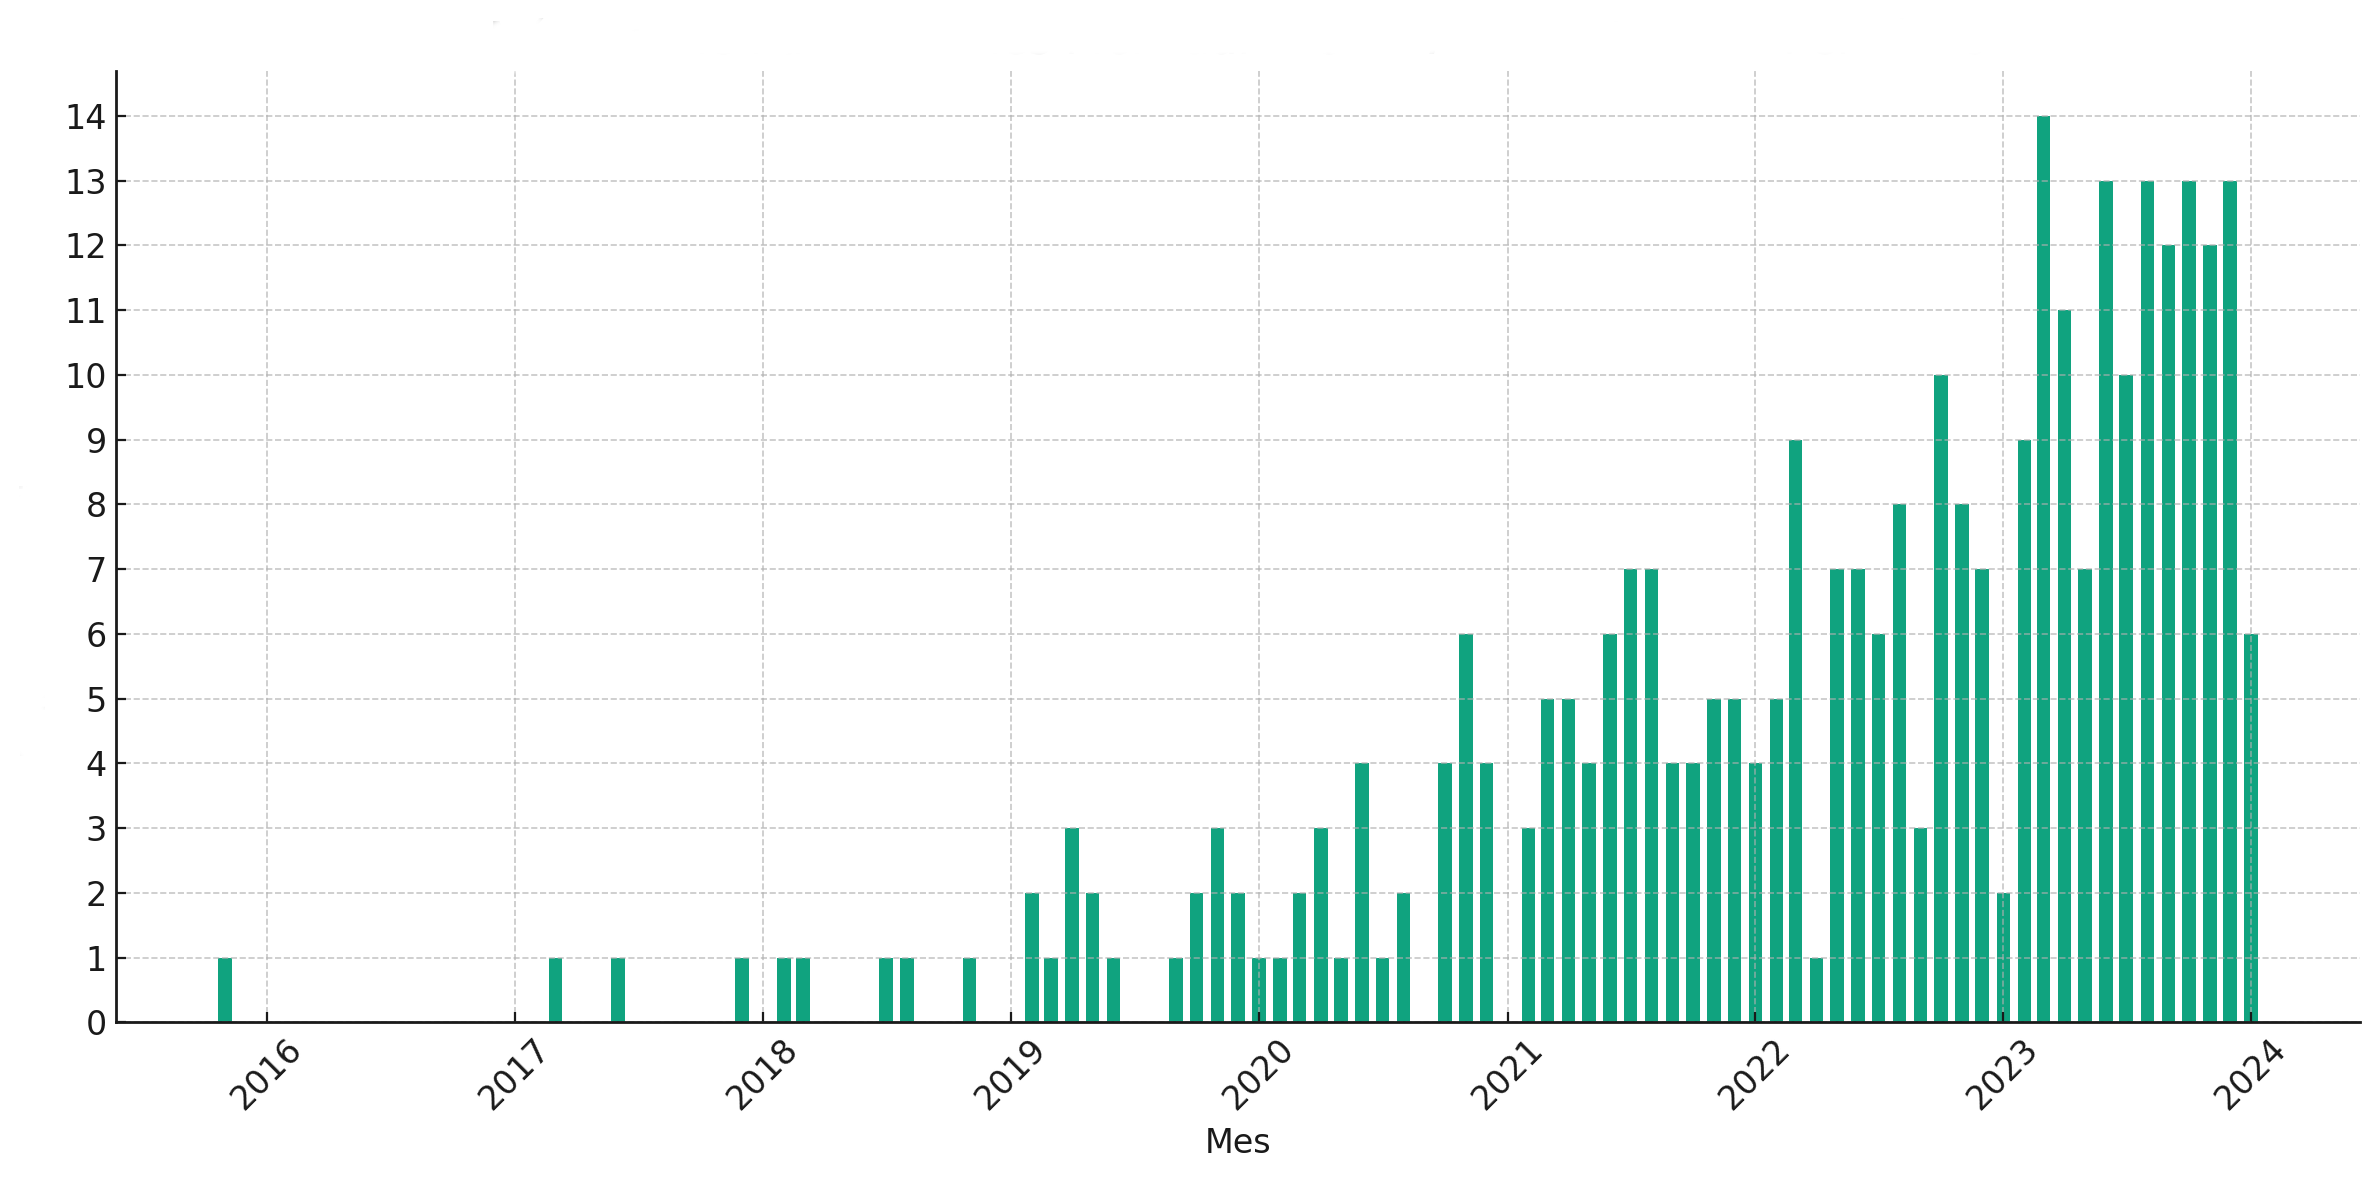
\includegraphics[width=0.7\textwidth]{./figuras/all_you_need_publicacionies_mensuales.png}
    \source{\propio\ a partir del listado de \cite{nishiKentoNishiAwesomeallyouneedpapers2024}}
    \label{fig:all_you_need_publicaciones}
\end{figure}



